\section{Datasample, Event Selection, and Noise Cleaning} \label{sec:EventSelection}

{\bf Dataset and CMSSW release:}
\begin{itemize}
\item dataset: /MinimumBias/Commissioning10-GOODCOLL-Jun9thSkim\_v1/RECO
\item CMSSW release: CMSSW\_3\_7\_0\_patch2
\end{itemize}

{\bf Event selection:}
\begin{itemize}
\item Physics declared bit
\item BPTX bit 0
\item Removal of events with large pixel cluster multiplicity
\item Good primary vertex
\item Good Run/LS selection. JSON file: Cert\_132440-136119\_7TeV\_May27thReReco\_Collisions10\_JSON.txt  
\end{itemize}
%More details at [XXX].

{\bf Noise cleaning}

Noise cleaning/event filter for calotower-based $\etmiss$ algorithms (Calo$\etmiss$ and tc$\etmiss$):
\begin{itemize}
\item ECAL barrel spikes (reject RecHits): topology (kWeird flag = swiss cross variable) + timing (kOutOfTime flag)~\cite{ECALAt7TeV};
\item HF PMT hits (reject Rechits): topology (HFLongShort flag = PET+S9/S1) + pulse shape (HFDigiTime flag)~\cite{HFDN};
\item HPD/RBX noise in HBHE (reject events): combination of pulse shape and topological variables~\cite{HCALWGNOTE}.
\end{itemize}

Noise cleaning (reject RecHits) for pf$\etmiss$ is described at~\cite{PFPAS2010}. Timing and topology are used to reject RecHits 
affected by ECAL and HF noise. Topology only is used to reject rechits affected by HBHE noise. No events are rejected.

NOTE: The HPD/RBX noise filter is applied for the scan of both tc$\etmiss$ and pf$\etmiss$ tails presented in this note, 
in order to have the same number of events passing the selection.

Figure~\ref{fig:calomet} shows the cleaned tc$\etmiss$ and pf$\etmiss$ distributions for $\approx 60$~M events 
(precisely 58821832 events) passing the event selection described above.
\begin{figure}[h]
 \centering
 \begin{tabular}{ll}
   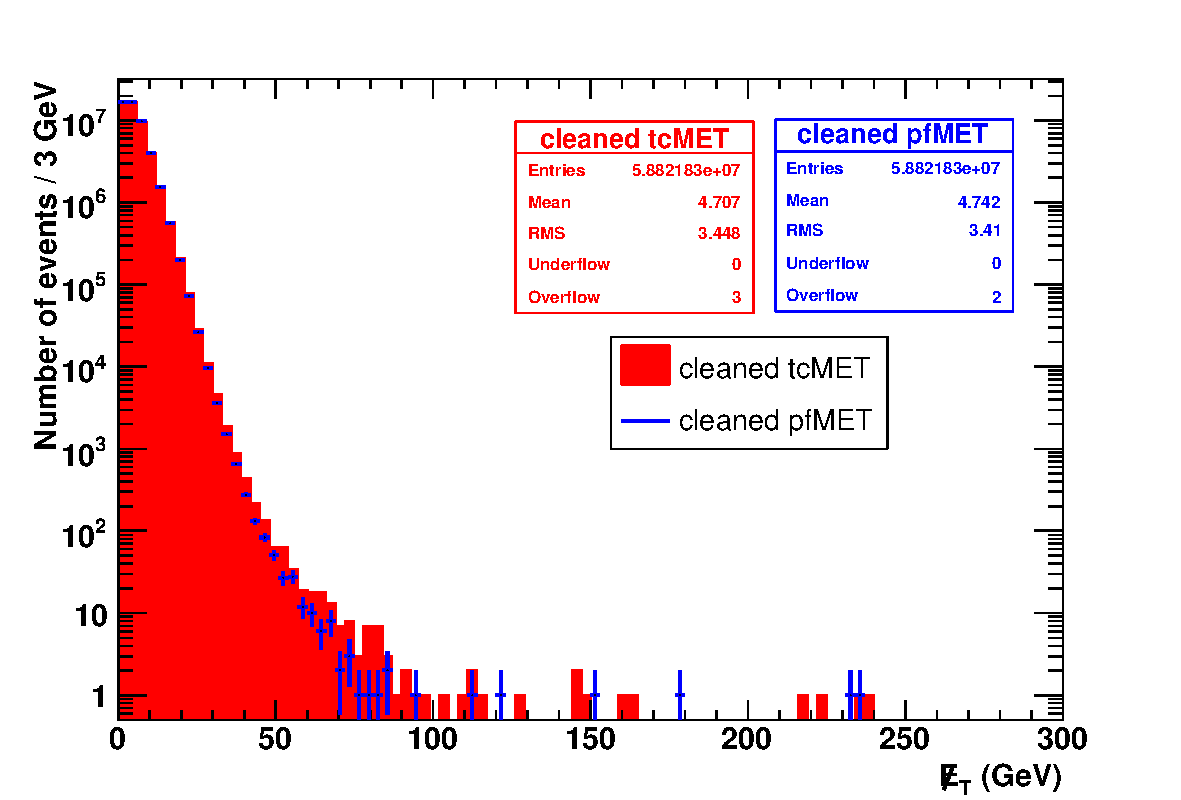
\includegraphics[width=0.7\textwidth]{fig/met.pdf} 
 \end{tabular}
\caption{tc$\etmiss$ and pf$\etmiss$ distributions of 7 TeV collision data after applying the full event selection and noise cleaning.}
\label{fig:calomet}
\end{figure}
